\documentclass{report}

\usepackage{authblk}
\usepackage{fancyhdr}
\usepackage{graphicx}
\usepackage{indentfirst}
\usepackage[portuguese]{babel}

\title{TP2}
\title{
    Comunicação por Computador \\
    \large{Trabalho Prático 3}
}

\author{
    Cristiano Pereira A93726 \\
    Marco Costa A93283 \\
    Hugo Fernandes A89481
}

\affil{
    Universidade do Minho \\
    Departamento de Informática
}


\begin{document}
    \maketitle
    \newpage

    \section*{Parte I}
        \subsection*{C}
            \noindent
            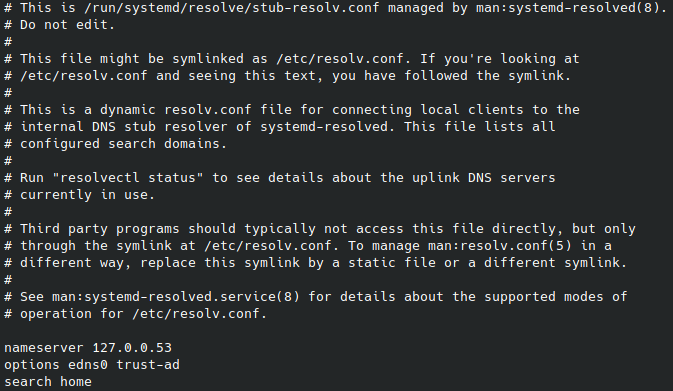
\includegraphics[width=\textwidth]{images/resolv.conf.png}
            \par
                O ficheiro \textit{/etc/resolv.conf} é lido pelas rotinas do resolver para saber
            a que servidor de DNS se deve conectar, bem como outras informações de configuração.\par 
                Na imagem acima pode ser visto todo o conteúdo deste ficheiro. Para além de várias linhas de comentários
            podem ser lidas três linhas que dizem ao \textit{resolver} como se comportar. Esta máquina foi configurada com os seguintes parâmetros: 
            \begin{description}
                \item[nameserver 127.0.0.53] Diz ao \textit{resolver} a que servidor DNS se deve conectar. Neste caso aponta para o endereço 127.0.0.53 no
                \textit{localhost} onde opera o processo \textit{systemd-resolved} que toma conta do processo de encaminhamento dos pedidos.
                \item[options edns0 trust-ad] Permite mudar as variáveis internas do \textit{resolver}.
                \item[search home]   
            \end{description}
        \pagebreak
        \subsection*{B}
                Através do programa \textit{dig} podemos fazer queries de DNS para saber se algum dos servidores \textbf{www.di.uminho.pt.} ou \textbf{www.europa.eu}
            tem algum endereço IPv6.\par
                Usamos o comando \textit{dig www.di.uminho.pt. AAAA} para procurar especificamente por endereços IPv6 e obtivemos a seguinte resposta:    
            \par
            \noindent
            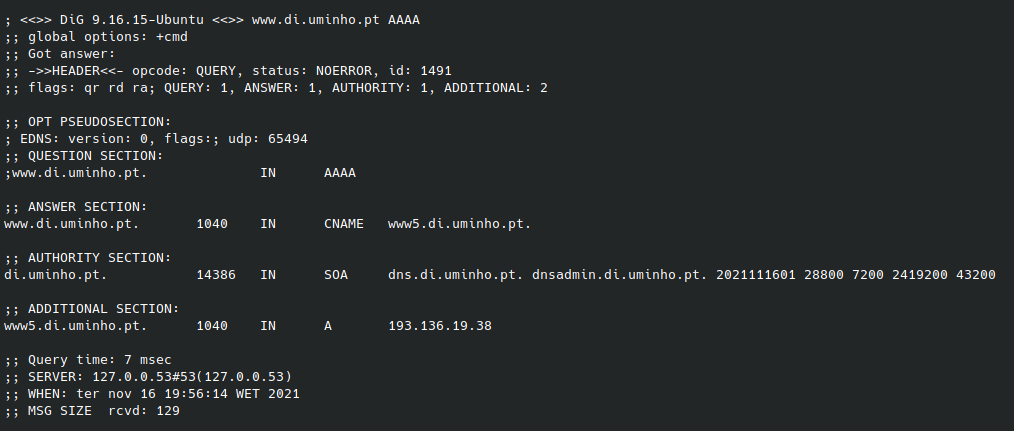
\includegraphics[width=\textwidth]{images/dig_di.png}
            \par
                A resposta que nos foi fornecida não inclui nenhuma entrada \textbf{AAAA} logo conluímos que este servidor não tem nenhum endereço IPv6.

                \vspace{0.45em}
                Por outro lado o output de \textit{dig www.europa.eu. AAAA} foi o seguinte:
            \par
            \noindent
            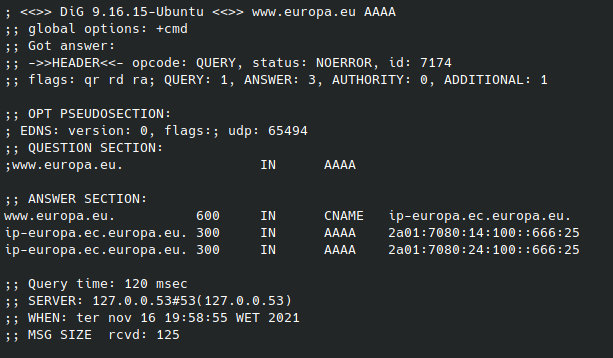
\includegraphics[width=\textwidth]{images/dig_europa.png}
            \par
                Esta resposta ao contrário da anterior mostra um \textbf{CNAME} que aponta para \textbf{ip-europa.ec.europa.eu.} e dois endereços IPv6 pertencentes a esse servidor.
        \pagebreak
        \subsection*{C}
            \noindent
            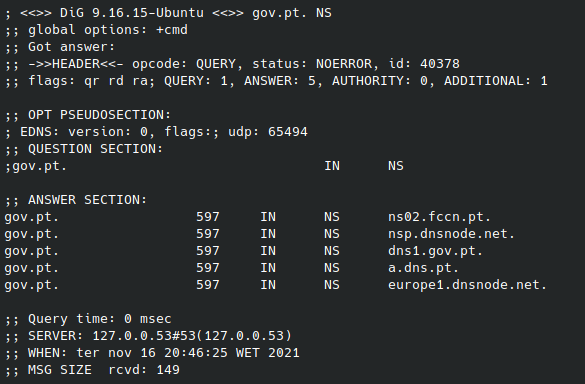
\includegraphics[width=\textwidth]{images/dig_gov.pt.png}
            \par
                Ao passarmos \textbf{NS} ao \textit{dig} podemos procurar pelos servidores de nome pertencentes ao domínio \textbf{gov.pt.} que nos retornou a imagem acima que contém o nome de cinco \textit{nameservers}.\par
            \noindent
            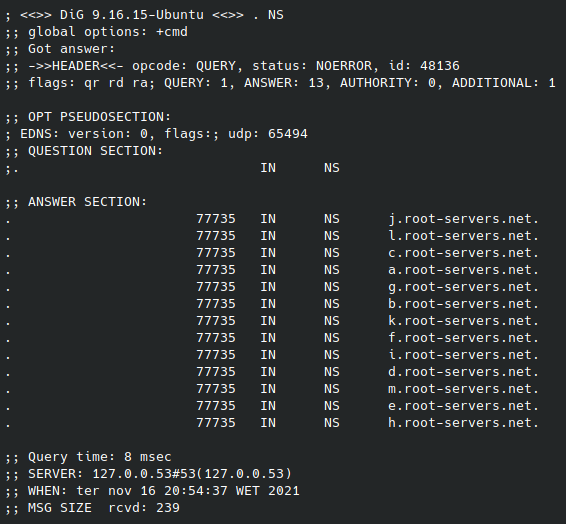
\includegraphics[width=\textwidth]{images/dig_root.png}
            \par
                Ao fazermos a mesma query relativamente ao servidor "." obtivemos o nome de todos os servidores \textbf{root} que como se pode ver na resposta foi-lhes atribuida uma letra a cada um.
        \pagebreak
        \subsection*{D}
                Para respondermos a esta questão usamos a flag \textbf{ANY} para procurar por todos os registos relativos a \textbf{efiko.academy.} e obtivemos a seguinte resposta:

            \vspace{0.45em}
            \noindent
            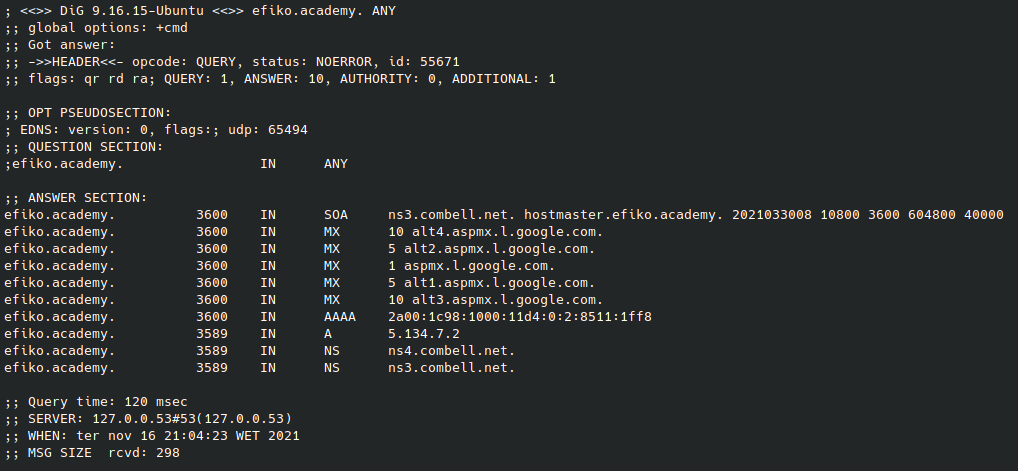
\includegraphics[width=\textwidth]{images/dig_efiko.png}
            \par

            \vspace{0.45em}
                Pelo registo \textbf{SOA} podemos concluir que este se trata de um domínio.
                Para além disso existem endereços IPv4 e IPv6 associados a este nome o que significa que \textbf{efiko.academy.} também é um host.
        \subsection*{E}
            \noindent
            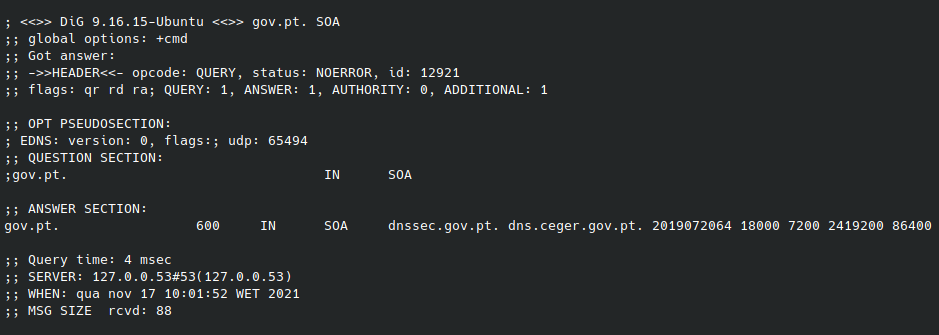
\includegraphics[width=\textwidth]{images/dig_gov_soa.png}
            \par
            
            O servidor dns principal pode ser encontrado através de uma query \textbf{SOA}.
            Assim podemos ver, entre outra informação, que o nome deste é \textbf{dnssec.gov.pt.}. Podemos também ver através das flags \textit{rd ra(recursion desired/recursion available)} que existe de facto recursividade disponível.
        \pagebreak
        \subsection*{F}
            A partir da query que foi feita na questão anterior podemos concluir que o servidor dns principal tem o nome \textbf{dnssec.gov.pt.}\par
            Com isto podemos procurar pelo seu endereço IPv4/IPv6:
            \par 
            \noindent
            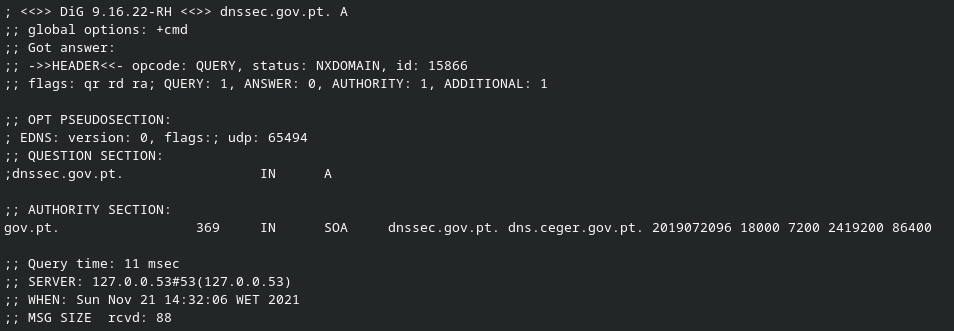
\includegraphics[width=\textwidth]{images/dig_dnssec_a.png}
            \par 
            \noindent
            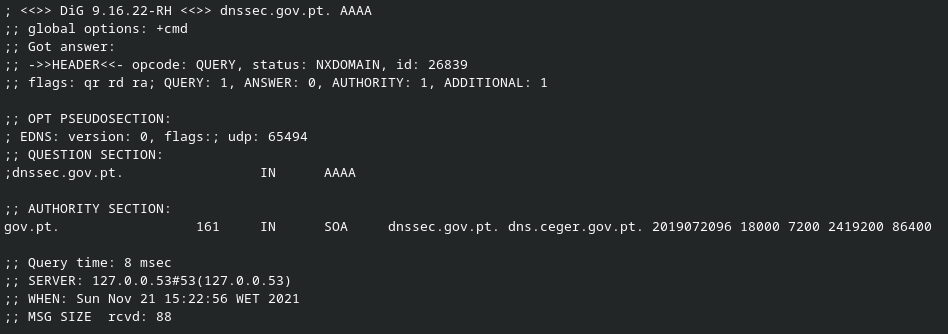
\includegraphics[width=\textwidth]{images/dig_dnssec_aaaa.png}
            \par
            Bem... Através destas queries descobrimos que este servidor não tem endereço IPv4 nem IPv6.
            Assim não conseguimos obter uma resposta autoritativa.
        \subsection*{G}
            \noindent
            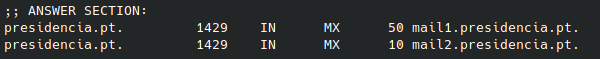
\includegraphics[width=\textwidth]{images/dig_presidencia.png}
            \par
            \noindent
            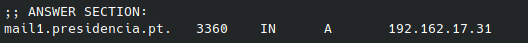
\includegraphics[width=\textwidth]{images/mail1_a.png}
            \par
            \noindent
            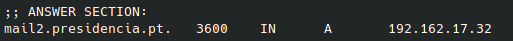
\includegraphics[width=\textwidth]{images/mail2_a.png}
            \par
            Ao fazermos uma query \textbf{MX} podemos ver os servidores de email pertencentes ao domínio presidencia.pt..\par
            Com esta resposta verifica-se a existência de dois destes servidores, \linebreak \textbf{mail1.presidencia.pt.} e \textbf{mail2.presidencia.pt.}, com endereços IPv4 \linebreak \textbf{192.162.17.31} e \textbf{192.162.17.32} respetivamente.
            Mais ainda podemos ver que mail2 tem prioridade superior devido ao valor de prioridade inferior.
        \subsection*{H}
            \noindent
            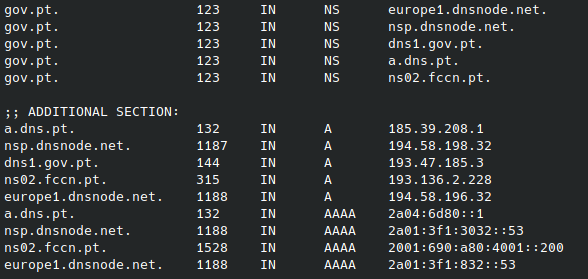
\includegraphics[width=\textwidth]{images/dig_gov_any.png}
            \par
            Para além de várias chaves de dns e assinaturas, ao procurarmos com a flag ANY, observamos que o domínio \textbf{gov.pt.} tem cinco servidores de dns diferentes, quatro deles com endereços IPv6 e todos com endereços IPv4.
        \subsection*{I}
            \noindent
            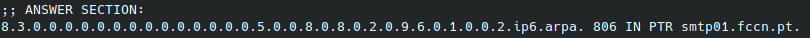
\includegraphics[width=\textwidth]{images/dig_ipv6.png}
            \par
            A resposta retornada pelo servidor de dns mostra um registo que aponta para o nome \textbf{smtp01.fccn.pt.}.
            Fazendo uma query a \textbf{smtp01.fccn.pt.} obtemos o endereço 193.137.198.38.
            \par
            \noindent
            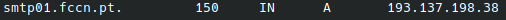
\includegraphics[width=\textwidth]{images/dig_smtp01.png}
            \par
        \subsection*{J}
            Os servidores secundários utilizam o registo \textbf{SOA} do servidor primário para atualizarem os seus registos. 
            Com a imagem seguinte podemos ver um exemplo de um destes registos: 
            \vspace{0.45em}
            \par
            \noindent
            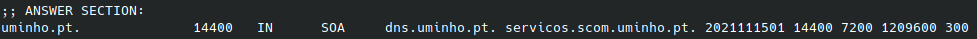
\includegraphics[width=\textwidth]{images/uminho_soa.png}
            \par
            \vspace{0.45em}
            De toda a informação apresentada os servidores utilizam as cinco últimas colunas para se atualizarem:
            \begin{description}
                \item[2021111501] Este é o número de serial que indica a versão da base de dados e que é alterado cada vez que a base de dados é alterada. 
                \par Os servidores secundários verificam este valor para saberem se se devem atualizar.
                \item[14400] Este valor indica o intervalo em que os servidores secundários devem fazer um novo pedido SOA.
                \item[7200] Caso o pedido SOA falhe este campo indica o tempo que o servidor deve esperar até enviar um novo pedido.
                \item[1209600] Se um servidor secundário não receber uma resposta do servidor primário durante este período de tempo este deve deixar de responder a queries para a zona
                \item[300] Este valor especifica o tempo que um cliente guarde os registos deste servidor na cache. 
            \end{description}


\end{document}